\setcounter{secnumdepth}{3}
\section{Moduł R\_PEAKS}
\subsection{Badania literaturowe}

Zadaniem modułu R\_PEAKS jest detekcja załamków R w elektrokardiogramie. Jest to jeden z kluczowych etapów analizy sygnału EKG. Poprawne wykrycie i oznaczenie załamków R umożliwia bowiem wykrycie pozostałych punktów charakterystycznych cyklu pracy serca. Pozwala to dalej np. na przeprowadzenie dokładnej analizy zmienności rytmu serca. Załamki R są częścią tzw. zespołu QRS, który został przedstawiony na rysunku \ref{fig:RPQRS}.
\begin{figure}[H]
\centering

\includegraphics[scale=0.7]{R_PEAKS/img/qrs_class}
\caption{Fragment sygnału EKG z zaznaczonym zespołem QRS (QRS Complex)}
\label{fig:RPQRS}
\end{figure}
Zespół QRS tworzą trzy sąsiadujące ze sobą punkty elektrokardiogramu, które składają się na wychylenie w kształcie wąskiego impulsu. Załamek Q to pierwsze ujemne wychylenie elektrokardiogramu, załamek R to pierwsze dodatnie wychylenie elektrokardiogramu, a załamek S to ostatnie ujemne wychylenie elektrokardiogramu w zespole QRS.

Zespół QRS jest odzwierciedleniem elektrycznej aktywności serca podczas skurczu komorowego. Reprezentuje on pobudzenie, czyli depolaryzację komór serca. Zespół QRS charakteryzuje się najwyższym wychyleniem i najkrótszym czasem trwania, co sprawia, że posiada on szerokie widmo częstotliwościowe. Charakterystyczny kształt tego zespołu oraz czas jego pojawiania się dostarcza najwięcej informacji diagnostycznych o bieżącym stanie serca i dlatego też jest punktem wyjściowym do klasyfikacji schematu cyklu sercowego. Służy też jako podstawa do automatycznego określania rytmu. Wykrycie zespołu QRS dostarcza podstawowych zasad i informacji dla prawie wszystkich automatycznych algorytmów analizy EKG. Czas trwania oraz wysokość zespołu QRS jest zależny od wielu czynników. Przyjmuje się jednak, że dla dorosłego i zdrowego człowieka średni czas trwania zespołu powinien wynosić od 0,06 s do 0,10 s. Wysokość sygnału zaś powinna mieścić się między 0,7 mV a 1,8 mV.

Detekcja załamków R wciąż jest przedmiotem wielu badań oraz licznych prac naukowych. Nie opracowano do tej pory metody, która gwarantowałaby stuprocentową skuteczność działania. Istnieją jednak algorytmy, które zapewniają ponad dziewięćdziesięciodziewięcio procentową skuteczność. Najpowszechniej stosowanym algorytmem jest algorytm Pan-Tompkins. Bazuje on na analizie odpowiednio przefiltrowanego oraz uśrednionego sygnału EKG. Algorytm ten łatwo adaptuje się do dynamiki sygnału. Dzięki temu jest bardzo skuteczny nawet w przypadku nieregularnej pracy serca. Ponadto metoda ta bardzo dobrze spisuje się w systemach czasu rzeczywistego. Wśród pozostałych algorytmów dużą popularnością cieszą się algorytmy oparte na przekształceniach Hilberta oraz transformacji falkowej. Przedmiotem obecnych badań są też metody, które łączyłyby te dwa algorytmy. Pozostałymi algorytmami detekcji załamków R są między innymi metody oparte na sieciach neuronowych, algorytmach genetycznych czy procesach stochastycznych.
\subsection{Koncepcja proponowanego rozwiązania}

W trakcie realizacji modułu R\_PEAKS zdecydowano się na implementację trzech algorytmów detekcji załamków R:
\begin{itemize}
\item algorytm Pan - Tompkins,
\item algorytm bazujący na przekształceniach Hilberta,
\item algorytm bazujący na transformacji falkowej.
\end{itemize}
\subsubsection{Algorytm Pan - Tompkins}

Algorytm ten można podzielić na dwa etapy. Pierwszym jest odpowiednie przygotowanie sygnału poprzez przefiltrowanie go oraz późniejsze jego uśrednienie. Drugim etapem jest znajdowanie załamków R we wcześniej przygotowanym sygnale. Na rysunku nr 2 przedstawiono schemat blokowy pierwszego etapu algorytmu.
\begin{figure}[H]
\centering
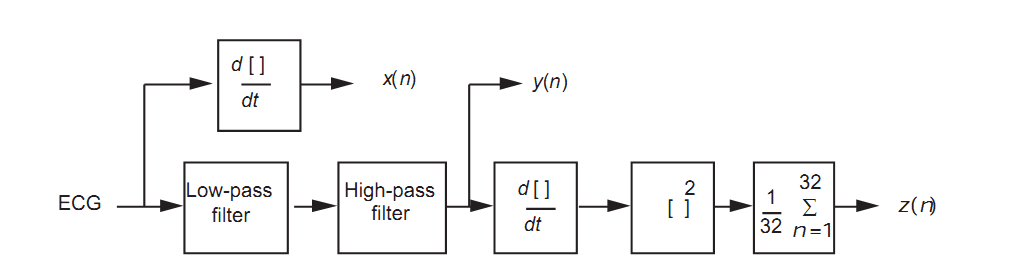
\includegraphics[scale=0.4]{R_PEAKS/img/pan_tompkins_alg}
\label{fig:RPPTA}
\caption{Kolejne etapy algorytmu Pan - Tompkins}
\end{figure}
Jako, że moduł R\_PEAKS otrzymuje już przefiltrowany sygnał od innego modułu, analiza poszczególnych faz algorytmu zacznie się od fazy różniczkowania.
\begin{enumerate}[I.]
\item Różniczkowanie

Celem różniczkowania sygnału jest wytłumienie komponentów niskoczęstotliwościowych oraz wzmocnienie komponentów wysokoczęstotliwościowych charakterystycznych dla zespołów QRS. W tej fazie skorzystano z różniczkowania pięciopunktowego opisanego wzorem:
\begin{equation}
y(nT)=\frac{1}{8}[-x(nT-2T)-2x(nT-T)+2x(nT+T)+x(nT+2T)]
\end{equation}
\item Potęgowanie

Potęgowanie sygnału ma na celu jeszcze większe wzmocnienie próbek sygnału odpowiadających zespołom QRS oraz wytłumienie pozostałych próbek sygnału. Ponadto potęgowania zapewnia nieujemność sygnału.
\begin{equation}
y(nT)=[x(nT)]^2
\end{equation}
\item Całkowanie

Całkowanie sygnału w ruchomym oknie ma na celu jego wygładzenie oraz uzyskanie pojedynczej "fali" w obrębie zespołu QRS. Całkowanie sygnału wyraża się następującym wzorem:
\begin{equation}
y(nT)=\frac{1}{N}\sum\limits_{i=nT-NT}^{nT} x(i)
\end{equation}
Gdzie N to szerokość okna, którą należy odpowiednio dobrać w zależności od częstotliwości próbkowania. Należy mieć tu na uwadze fakt, że zbyt duża wielkość okna spowoduje zlanie się dwóch fal, a zbyt mała z kolei skutkować będzie utworzeniem zbyt dużej liczby fal.
\item Progowanie i detekcja załamków R

W trakcie pracy algorytmu odnajdywane są kolejne maksima lokalne, którą mogą być oznaczone jako załamek R lub jako szum. Wykorzystywane są przy tym dwa progi: THRESHOLD1 i THRESHOLD2. Są one na bieżąco aktualizowane na podstawie estymaty amplitudy załamków R (SPK) i szumu (NPK). Dodatkowo wykorzystywana jest technika searchback z parametrem RRMISSEDLIMIT, który wyznaczany jest na podstawie różnic między kolejnymi załamkami R. Poniżej przedstawiono reguły detekcji załamków R:
\begin{itemize}
\item Jeżeli nowy załamek R wykryto w czasie maksymalnie 200 ms od ostatniego załamka R i amplituda nowego załamka jest mniejsza od poprzedniego wykrytego to ten załamek jest odrzucany.
\item Jeżeli nowy załamek R wykryto w czasie ponad 200 ms, a mniej niż 360 ms od ostatniego załamka sprawdza się, czy maksymalne nachylenie sygnału przy nowym maksimum jest przynajmniej równe połowie nachylenia dla poprzedniego maksimum. Jeżeli nie, to przyjmuje się, że maksimum jest szumem, np. załamkiem T.
\item Jeżeli wartość wykrytego maksimum jest większa niż THRESHOLD1, to uznaje się to maksimum za załamek R, w przeciwnym razie jest to szum.
\item Technika searchback: Jeżeli załamek R nie został wykryty przez okres RRMISSEDLIMIT, a w ciągu tego czasu zostały znalezione maksima większe niż THRESHOLD2, to największe z nich traktowane jest jako załamek R.
\end{itemize}
W takcie działania algorytmu konieczna jest aktualizacja progów. Są one aktualizowane na podstawie wartości parametrów SPK i NPK, których początkowe wartości są następujące:
\begin{itemize}
\item SPK = średnia z ośmiu maksimów z pierwszych ośmiu sekund badania,
\item NPK = 0.
\end{itemize}
Wartości tych parametró są aktualizowane w następujący sposób:
\begin{itemize}
\item jeżeli załamek R został wykryty za pomocą porównania z THRESHOLD1 
\newline
SPK = 0.125 PEAK + 0.875 SPK,
\item jeżeli załamek R został wykryty za pomocą porównania z THRESHOLD2 
\newline
SPK = 0.250 PEAK + 0.750 SPK,
\item jeżeli został wykryty szum
\newline
NPK = 0.125 PEAK + 0.875 NPK
\end{itemize}
Progi natomiast są aktualizowane w następujący sposób:
\newline
THRESHOLD1 = NPK+ 0.25 (SPK-NPK)
\newline
THRESHOLD2 = 0.5 THRESHOLD1

Interwały pomiędzy kolejnymi załamkami R obliczane są jako różnica wystąpienia ich czasów. Jeżeli interwał jest większy niż 0.92 RRAVERAGE2 i mniejszy niż 1.12 RRAVERAGE2, bufor interwałów jest aktualizowany o ostatnią wartość interwału i obliczana jest nowa wartość RRAVERAGE2. Wartość RRMISSEDLIMIT używana w technice searchback jest równa 1.66 RRAVERAGE2 i stanowi czas, w którym poszukiwane są zaginione maksima.
\end{enumerate}
\subsubsection{Algorytm bazujący na przekształceniach Hilberta}
Przekształcenie Hilberta to przekształcenie liniowe. Funkcji x(t) przypisywana jest funkcja xh(t) postaci:
\begin{equation}
x_H = \mathcal{H}\{x(t)\}=\frac{1}{\pi}\int_{-\infty}^\infty \frac{x(\lambda)d\lambda}{t-\lambda}
\end{equation}
W powyższym wzorze występuje dość trudna do wyliczenia niewłaściwa całka Riemanna. W takiej sytuacji należy skorzystać z transformaty Fouriera. Wzór na przekształcenie Hilberta przyjmuje wtedy postać:
\begin{equation}
x_H(t)=Im \{ \mathcal{F}^{-1} \{ \mathcal{F} \{ x(t) \}(\omega)\cdot (-j)sgn(\omega)\}  \}
\end{equation}
W pierwszym etapie algorytmu dokonujemy transformacji Hilberta całego sygnału EKG. Następnie na podstawie sygnałów x(t) oraz xh(t) wyznacza się tzw. obwiednię sygnału postaci:
\begin{equation}
\mathcal{B}(t)=\sqrt{x(t)^2+x_H(t)^2}
\end{equation}
Po wyznaczeniu obwiedni sygnału należy przystąpić do etapu progowania.

\begin{enumerate}[I.]
\item Wyznaczenie początkowej wartości progu

Pierwsza wartość progu powinna być nieco mniejsza niż maksymalna wartość sygnału B(t). Najczęściej spotykana wartość progu to ok. 0,9 wartości maksymalnej sygnału B(t).
\item Wyznaczenie wartości o jaką należy zmniejszać próg w kolejnych iteracjach

Jeżeli za M1 przyjęto maksymalną wartość sygnału B(t), a za M2 wartość minimalną tego sygnału to wartość o jaką należy zmniejszać próg w każdej iteracji wyraża się następującym wzorem:
\begin{equation}
fi=0,01\cdot M1 \cdot x \cdot mantysa(M1-M2)
\end{equation}
\item Wyznaczenie załamków

W tym kroku należy wyliczyć ile próbek sygnału B(t) jest większych od obecnego progu. Jeżeli liczba próbek powyżej progu jest większa od ilości próbek w poprzedniej iteracji to należy zmniejszyć próg o wartość fi i ponownie policzyć próbki powyżej progu. Jeżeli ilość próbek powyżej progu się nie zmieniła to należy przerwać etap progowania.

Ostatnim etapem jest detekcja załamków R. Wyznaczone w etapie progowania próbki powyżej progu będą występować w grupach. W każdej z tych grup znajdować się będzie próbka o największej amplitudzie, która będzie szukanym załamkiem R.
\end{enumerate}
\subsubsection{Algorytm bazujący na transformacji falkowej}

Falki (z ang. wavelet) – rodziny funkcji zbioru liczb rzeczywistych w zbiór liczb rzeczywistych, z których każda jest wyprowadzona z funkcji-matki (z tzw. funkcji macierzystej) za pomocą przesunięcia i skalowania:
\begin{equation}
\psi_{j,k}(t)=\psi(2^j +k)
\end{equation}
gdzie: j,k – liczby całkowite, $\psi$ – funkcja - matka, $\psi_{j,k}$ – falka o skali j i przesunięciu k (zwana też funkcją falkową). Funkcje te dążą do zera lub po prostu wynoszą zero dla argumentów dążących do nieskończoności. Ponadto funkcje te mają energię skupioną w jednym miejscu tzn.
\begin{equation}
\int\limits_{-\infty}^{\infty} \psi(t)dt=0
\end{equation}
Transformacja falkowa dla sygnałów ciągłych jest przekształceniem całkowym:
\begin{equation}
\tilde{s}_{\Psi}=\frac{1}{\sqrt{a}}\int\limits_{-\infty}^{\infty}s(t)\Psi(\frac{t-b}{a})dt
\end{equation}
gdzie:
\begin{itemize}
\item a - parametr skali
\item b - parametr przesunięcia
\item s(t) - sygnał badany zależny od czasu t
\item $\Psi$ - funkcja falkowa
\item $\tilde{s} _\Psi$ - współczynnik falkowy zależny od parametrów a i b
\item $\Psi(\frac{t-b}{a})$ - jądro przekształcenia
\end{itemize}
Zastosowanie transformacji falkowej pozwala rozłożyć sygnał na kilka subpasm (rysunek \ref{fig:RPWS}). Następnie dobiera się odpowiednie subpasma i rekonstruuje sygnał. Tak uzyskany sygnał poddaje się takiej samej procedurze progowania i detekcji załamków R jak w przypadku wcześniej opisywanego algorytmu wykorzystującego przekształcenia Hilberta.
\begin{figure}[H]
\centering
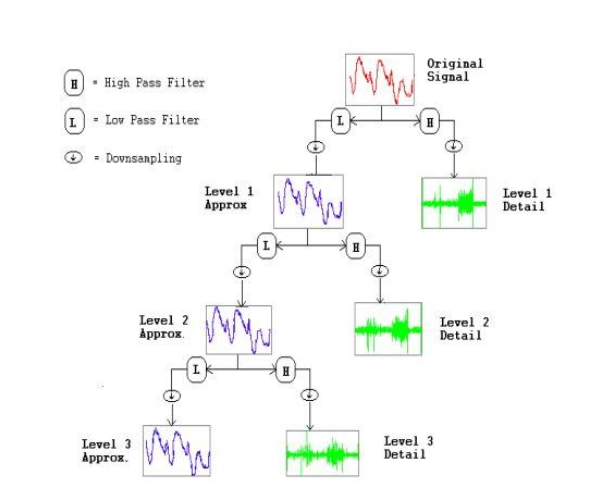
\includegraphics[scale=0.6]{R_PEAKS/img/wavelet_schema}
\caption{Dekompozycja sygnału na subpasma za pomocą transformacji falkowej}
\label{fig:RPWS}
\end{figure}
\subsection{Rezultaty i wnioski}
\subsection{Literatura}